\chapter{実装}
\label{implementation}

本章では本研究における実装環境,提案手法の実装,提案手法の評価に用いるデータセットについて述べる.
\ref{impl_env}では本研究における実験のための実行環境及び事前知識について述べる。
\ref{exp1}ではK-AFの性能を既存の活性化関数と比較する実験を行う。
\ref{exp2}では各データセットにおいての活性化関数の形を調査する実験をこなう。
\ref{exp3}では、K-AFの性能を最も引き出す可能性がある、学習の設定を調査する。



\section{実装環境}
\label{impl_env}



本研究において利用した実装環境を \ref{impl_table} に示す. 提案手法の実装は Pytorch 及
を用いた.  PyTorch~\cite{pytorch}, Chainer~\cite{chainer},  Tensorflow~\cite{tensorflow} は計算グラフの自動微分ライブラリであり, 深層ニューラルネットワークの研究や開発にも用いられる.
Pytorchを用いた理由は実装コストが低く研究領域に従事できるところにある。


\begin{table}[htbp]
\label{impl_table}
    \begin{center}
        \caption{本研究の実行環境}
        \vspace{5mm} 
        \begin{tabular}{l*{2}{c}r}
        ソフトウェア              & バージョン \\
        \hline
        Python            & 3.8.5  \\
        CPU               & Intel core i7  \\
        PyTorch           & 6 \\
        \end{tabular}
    \end{center}
\end{table}



\vspace{-15mm} 
\section{実験1}
\label{exp1}

実験に用いる活性化関数の形を図\ref{k-af-net}に示す。
\begin{figure}[hbtp]
\label{k-af-net}
    \begin{center}
        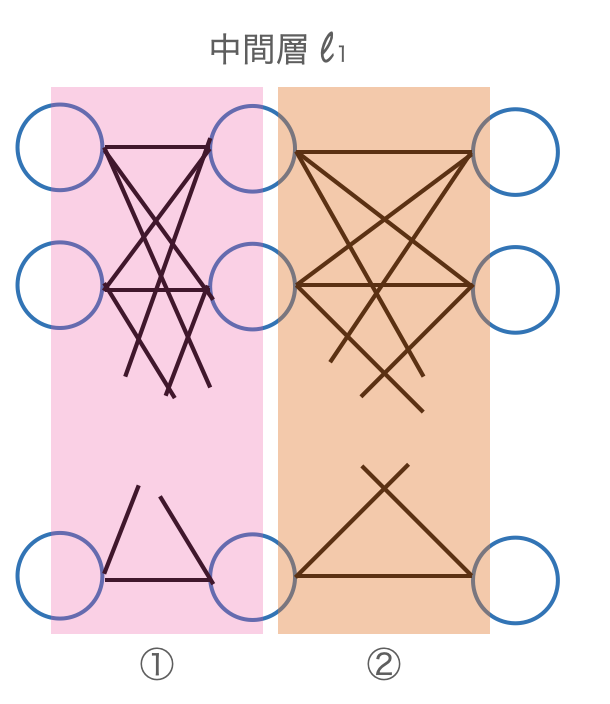
\includegraphics[width=10cm]{asset/k-af-net.png}
            \caption{実験で使うニューラルネットワークの概要図}
            \label{neural_network1}
    \end{center}
\end{figure}

今回の実験では、簡易的なモデルで活性化関数の性能を試していく。
中間層の数を$ l_1 $とし、\textcircled{\scriptsize 1}にはReLUを用いる。\textcircled{\scriptsize 2}の部分を可変的にさまざまな活性化関数へと変えていく。
本論文で提案する、K-AFは\textcircled{\scriptsize 2}の部分において性能を評価する。

比較用の活性化関数には以下を用いる。
\begin{itemize}
    \setlength{\parskip}{0cm} % 段落間
    \setlength{\itemsep}{0cm} % 項目間
    \item ReLU
    \item Sigmoid
    \item Linear
    \item TanH
    \item Mish
    \item Swish
    \item K-AF(本手法)
\end{itemize}


活性化関数の性能の比較実験のために、以下の項目を変えながら実験する。データセットにはsckit-learn~\cite{scikit-learn}のライブラリのデータセットに対してデフォルトで入ってるものを想定する。
\begin{itemize}

    \setlength{\parskip}{0cm} % 段落間
    \setlength{\itemsep}{0cm} % 項目間
    \item ラーニングレート [ $10^{-5}$, $10^{-6}$ ,$10^{-7}$]
    \item 初期値 [ Xavier, kaiming uniform]
    \item レギュラライザー [ 何もなし, L1ノルム, L2ノルム]
    \item optimizer [ SGD, Momentum, AdaGrad, Adam]
    \item データセット [ アヤメ, MNIST, wine, 住宅の価格, 健康の状態]
\end{itemize}



\subsection{比較データ}

他の活性化関数と適当に比較するために、以下の条件を比較して実験を行う。


\begin{table}[htbp]
    \begin{center}
        \caption{実験のデータセットの名称}
        \vspace{5mm} 
        \begin{tabular}{l*{2}{c}r}
        データセット名      & 出力層 & 出力の形式 & 中間層の数 \\
        \hline
        iris            & 3  & 分類 & 10  \\
        MNIST               & i10 & 分類 & 10   \\
        wine        & 13 & 分類 & 10  \\
        住宅の価格           & 6 & 回帰 & 10  \\
        健康の状態           & 6 & 回帰 & 10  \\
        膵臓癌           & 6 & 回帰 & 10  \\
        \end{tabular}
    \end{center}
\end{table}




\section{実装における留意点}
本研究における提案手法を実装する際に留意する必要のある点を述べる.
一つは勾配が消失してしまった場合の処理である。



\subsection{実験1}
\section{実装手法}


\section{活性化関数}




\section{実験2}
\label{exp2}
2つ目の実験では推論した活性化関数の形を観測し、既存の活性化関数との違いを定性評価を行う
\subsection{比較データ}


\section{実験3}
\label{exp3}
K-AFにおける学習の難点である、勾配消失について定量評価を行う。
\subsection{比較データ}


%%% Local Variables:
%%% mode: japanese-latex
%%% TeX-master: "../bthesis"
%%% End:
